\section{Monsterteam}\label{sec:monster-team}
Mit der Einführung der Funktion des Monsterteams ist die Verwaltung und die Übersicht der Monster leicht gemacht. 
Der Nutzer kann jederzeit seine Monster zum aktiven Team hinzufügen, entfernen und beliebig anordnen. 
Darüber hinaus kann der Nutzer die Monsterdetails des jeweiligen Monsters abrufen.
\subsection{Mockups}\label{subsec:mockups-monster-team}
Auf das Fenster des Monsterteams gelangt der Nutzer, wenn im Spielbildschirm der Knopf 'Monsters' gedrückt wird. 
Dabei erscheint zuerst der Inhalt der Registerkarte 'Active Team', in der das aktive Monsterteam wie in Abbildung~\ref{fig: Aktive Monster} dargestellt wird.
Alle Monster im aktiven Team haben den gleichen Aufbau: Das Monsterbild wird links angezeigt, dann folgen der Name, das Level und der Monster-Typ dieses Monsters.
Zudem gobt es vier Knöpfe wie in der Abbildung~\ref{fig: Aktive Monster} zu sehen ist: zwei Anordnungsknöpfe für die Reihenfolge der Monster, ein Knopf für das Entfernen aus dem aktiven Team und ein Knopf für das Anzeigen der Monsterdetails.
\begin{figure}[H]
    \center
    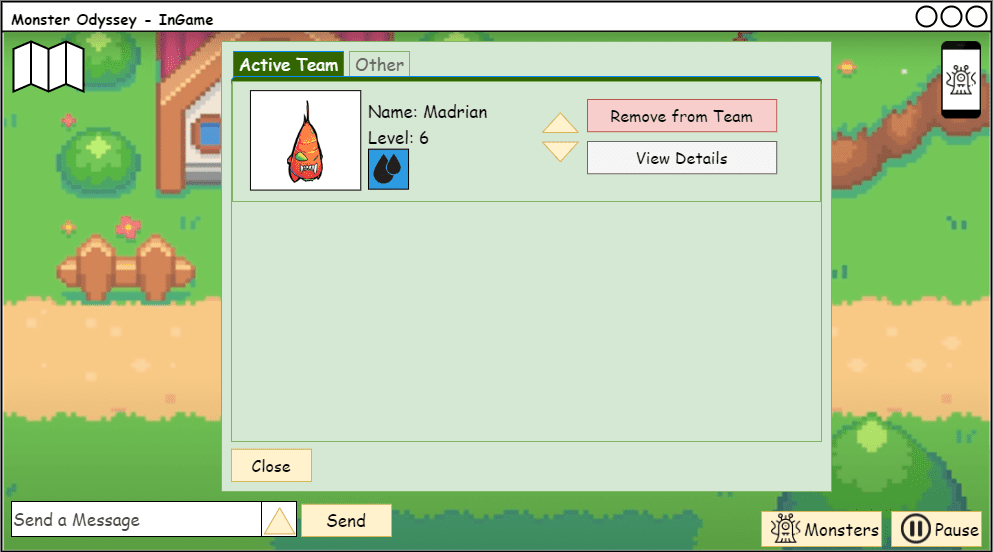
\includegraphics[scale=\scale]{images/mockups/Monster/IngameMonsterMonsterActiveWithoutFlamurtle.png}
    \caption{Mockup: Aktives Monsterteam}
    \label{fig: Aktive Monster}
\end{figure}
Zum Anzeigen der anderen Monster kann der Nutzer auf die Registerkarte 'Other' drücken. 
Dann wird der Inhalt des Fensters wie in Abbildung~\ref{fig: Andere Monster} aktualisiert, sodass die im aktiven Team nicht vorhandenen Monster angezeigt werden. 
Hier haben alle Monster den gleichen Aufbau wie im aktiven Team -- mit zwei klaren Unterschieden wie in den Abbildungen~\ref{fig: Aktive Monster} und~\ref{fig: Andere Monster}: Der 'Entfernen'-Knopf wird durch den 'Hinzufügen'-Knopf ersetzt und die Anordnungsknöpfe werden nicht angezeigt.
\begin{figure}[H]
    \center
    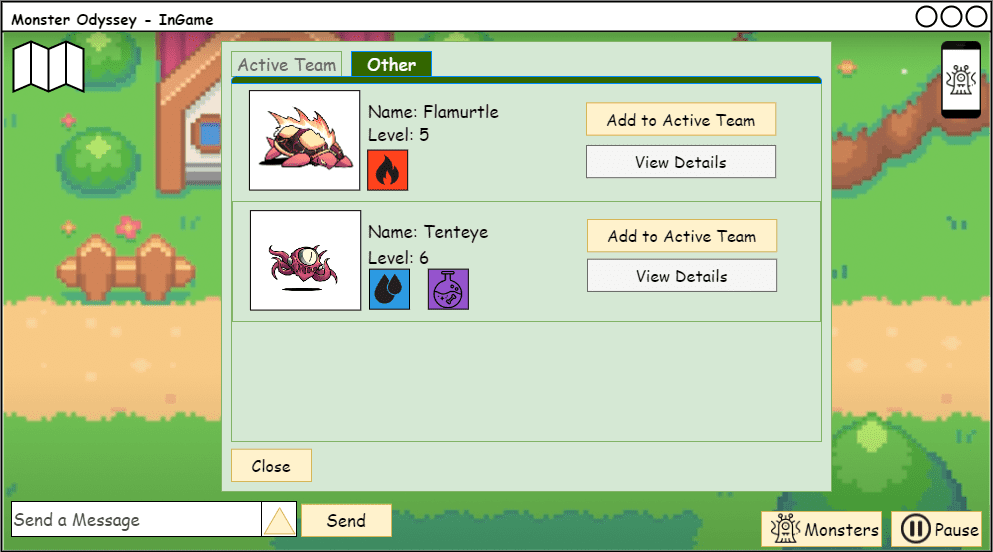
\includegraphics[scale=\scale]{images/mockups/Monster/IngameMonster.png}
    \caption{Mockup: Andere Monster}
    \label{fig: Andere Monster}
\end{figure}
Die Details von dem jeweiligen Monster können durch Drücken des Knopfs 'View Details' aufgerufen und angezeigt werden. Es erscheint das Fenster wie in der Abbildung~\ref{fig: Monsterdetails}. Der Aufbau der Monsterdetails folgt demselben Schema wie in der Abbildung~\ref{fig: Informationen über den jetzigen Monster}. In diesem Fall können für ein beliebiges Monster die Informationen abgerufen werden.
\begin{figure}[H]
    \center
    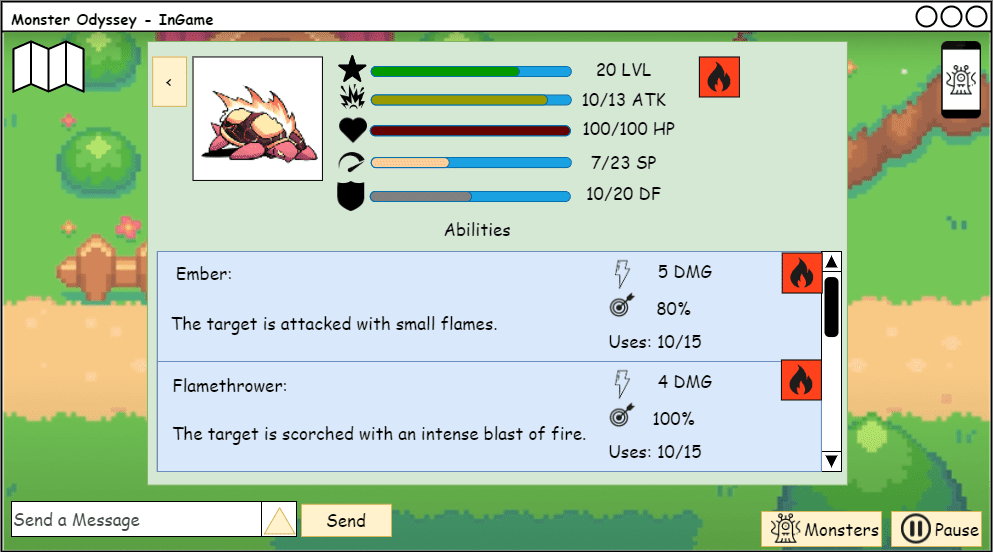
\includegraphics[scale=\scale]{images/mockups/Monster/IngameMonsterDetails.png}
    \caption{Mockup: Monsterdetails}
    \label{fig: Monsterdetails}
\end{figure}
Der Nutzer kann weiterhin ein beliebiges Monster zum aktiven Monsterteam beim Drücken des Knopfs 'Add to Active Team' hinzufügen. 
Es erscheint dabei ein Popup für die Bestätigung wie in Abbildung~\ref{fig: Monster zum aktiven Team hinzugefügt} und das gewählte Monster wird in die Registerkarte des aktiven Teams verschoben.
Jedoch besteht die Möglichkeit, dass das aktive Monsterteam bereits die maximale Anzahl von sechs Monstern besitzt. 
Dann erscheint wie in Abbildung~\ref{fig: Max. Limit Aktiven Teams} beim Drücken desselben Knopfs die Fehlermeldung, dass das gewählte Monster nicht zum aktiven Team hinzugefügt werden konnte.
\begin{figure}[H]
    \center
    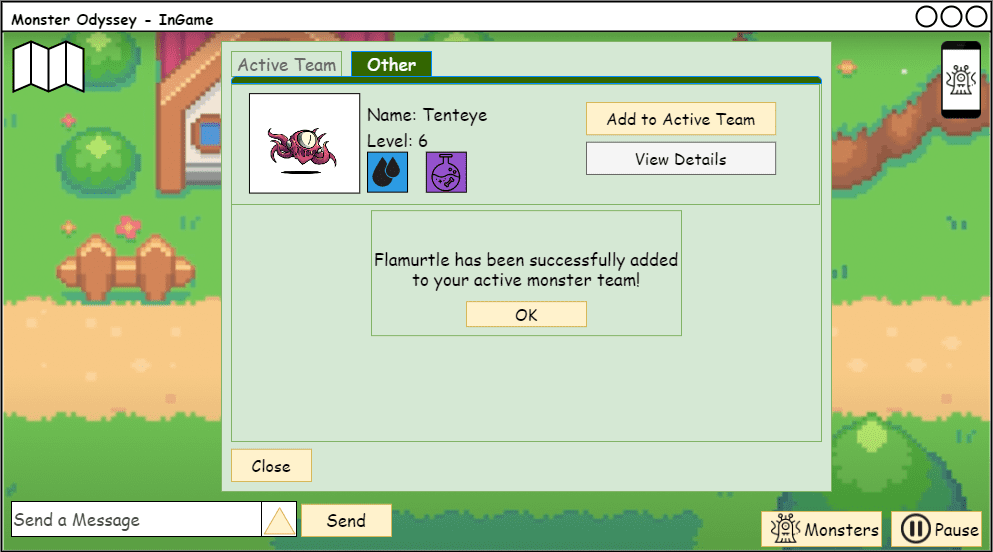
\includegraphics[scale=\scale]{images/mockups/Monster/IngameMonsterMonsterAdded.png}
    \caption{Mockup: Monster zum aktiven Team hinzugefügt}
    \label{fig: Monster zum aktiven Team hinzugefügt}
\end{figure}
\begin{figure}[H]
    \center
    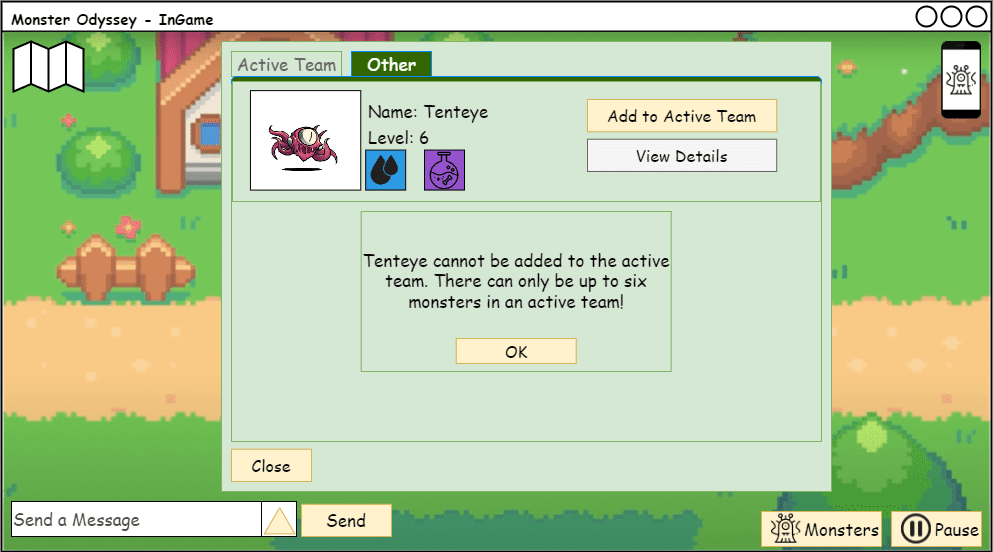
\includegraphics[scale=\scale]{images/mockups/Monster/IngameMonsterMonsterAddedMax.png}
    \caption{Mockup: Max. Limit Aktiven Teams}
    \label{fig: Max. Limit Aktiven Teams}
\end{figure}
Die Anordnung der Monster im aktiven Team besitzt eine relevante Rolle im Kampf. 
Das erste Monster in der Liste wird beim Kampfstart zum jetzigen Monster gesetzt. Hierdurch kann der Nutzer diese Eigenschaft mithilfe der Anordnung bevorzugt ausnutzen. 
Mit dem oberen Pfeilknopf kann das jeweilige Monster höher in der Liste gesetzt werden. Analog kann das jeweilige Monster mit dem unteren Pfeilknopf in der Liste weiter unten gesetzt werden. Die Abbildung~\ref{fig: Anordnung der Monster im aktiven Team} veranschaulicht, dass ein Monster aus der Abbildung~\ref{fig: Ursprüngliches aktives Team} eine Position nach unten gesetzt wird. Dadurch sieht das Ergebnis der Anordnung wie in Abbildung~\ref{fig: Anordnung geändert} aus.
\begin{figure}[H]
    \centering
    \begin{subfigure}[b]{0.4\textwidth}
        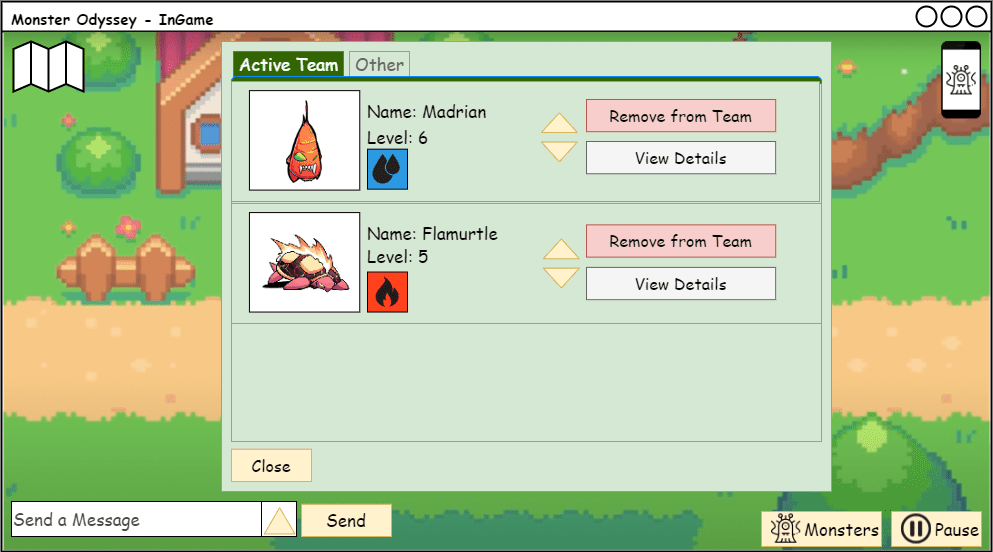
\includegraphics[width=\textwidth]{images/mockups/Monster/IngameMonsterMonster.png}
        \caption{Ursprüngliches aktives Team}
        \label{fig: Ursprüngliches aktives Team}
    \end{subfigure}
    \hfill
    \begin{subfigure}[b]{0.4\textwidth}
        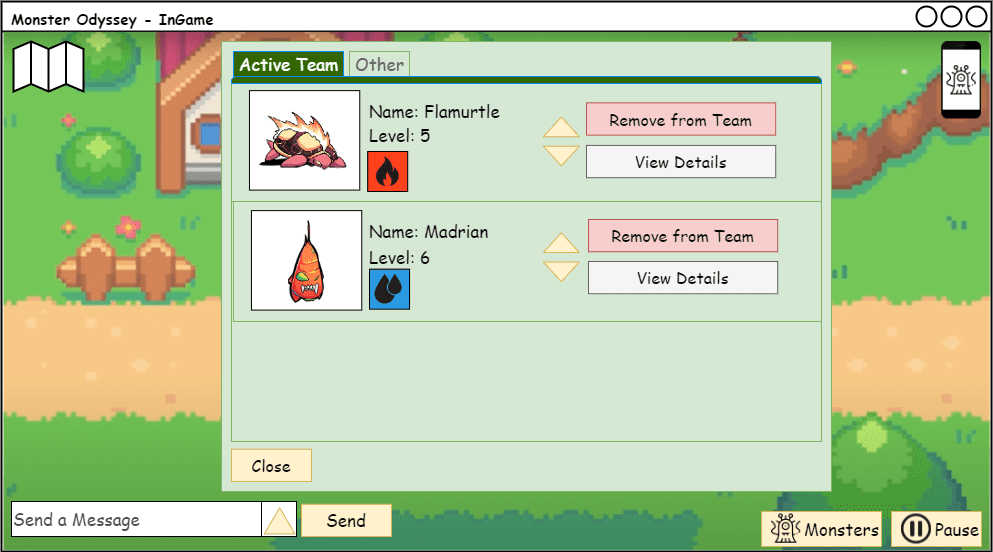
\includegraphics[width=\textwidth]{images/mockups/Monster/IngameMonsterMoved.png}
        \caption{Anordnung geändert}
        \label{fig: Anordnung geändert}
    \end{subfigure}
    \caption{Mockup: Anordnung der Monster im aktiven Team}
    \label{fig: Anordnung der Monster im aktiven Team}
\end{figure}
Analog zum Hinzufügen von Monstern in das aktive Team kann der Nutzer beliebige Monster aus dem aktiven Team entfernen. 
Auf der Registerkarte 'Active Team' kann der Nutzer dies tun, indem er den Knopf 'Remove from Team' wie in Abbildung~\ref{fig: Ursprüngliches aktives Team} drückt. Infolgedessen erfolgt ein Popup wie in Abbildung~\ref{fig: Monster vom aktiven Team entfernt}, indem die Aktion bestätigt wird. 
\begin{figure}[H]
    \center
    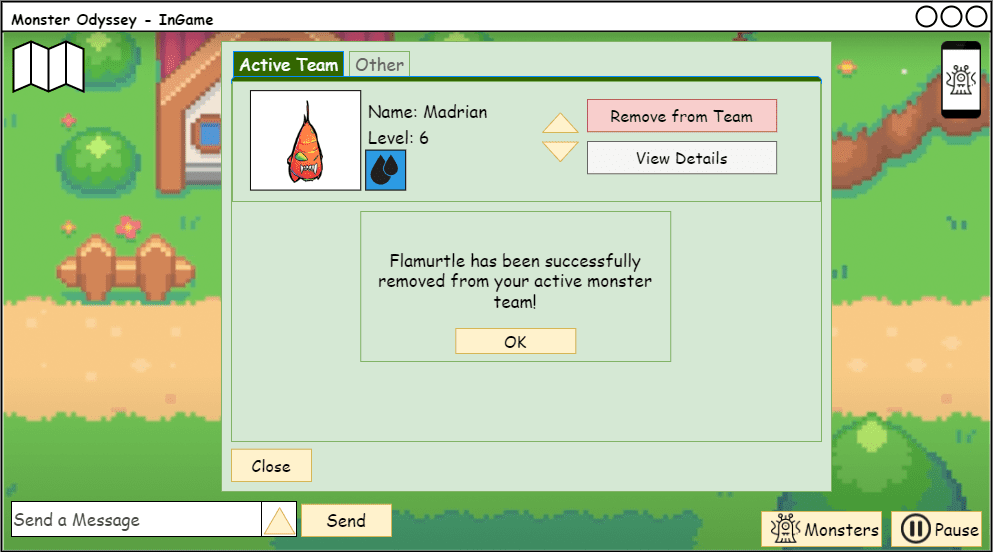
\includegraphics[scale=\scale]{images/mockups/Monster/IngameMonsterMonsterActiveRemoved.png}
    \caption{Mockup: Monster vom aktiven Team entfernt}
    \label{fig: Monster vom aktiven Team entfernt}
\end{figure}
\subsection{Vergleich zwischen Mockups und Implementierung}\label{subsec:vergleich-zwischen-mockups-und-implementierung-monster-team}
In der Abbildung~\ref{fig: Vergleich: Monsterliste} bestehen grundsätzlich keine wesentlichen Unterschiede. Allerdings sind mehrere Elemente aus dem Mockup aus der Abbildung~\ref{fig: Mockup: Aktives Monsterteam} nicht vorhande. Demnach existieren beispielsweise die grüne Trennlinie unter den Registerkarten, die Umrandung um die Monsterliste und der weiße Hintergrund in der Implementierung aus der Abbildung~\ref{fig: Implementierung: Aktives Monsterteam} nicht. Diese Unterschiede dienen der Ästhetik und haben keine semantischen Konsequenzen auf das Spiel. Sie sind aufgrund von Zeitproblemen und niedriger Priorität nicht implementiert worden.
\begin{figure}[H]
    \centering
    \begin{subfigure}[b]{0.4\textwidth}
        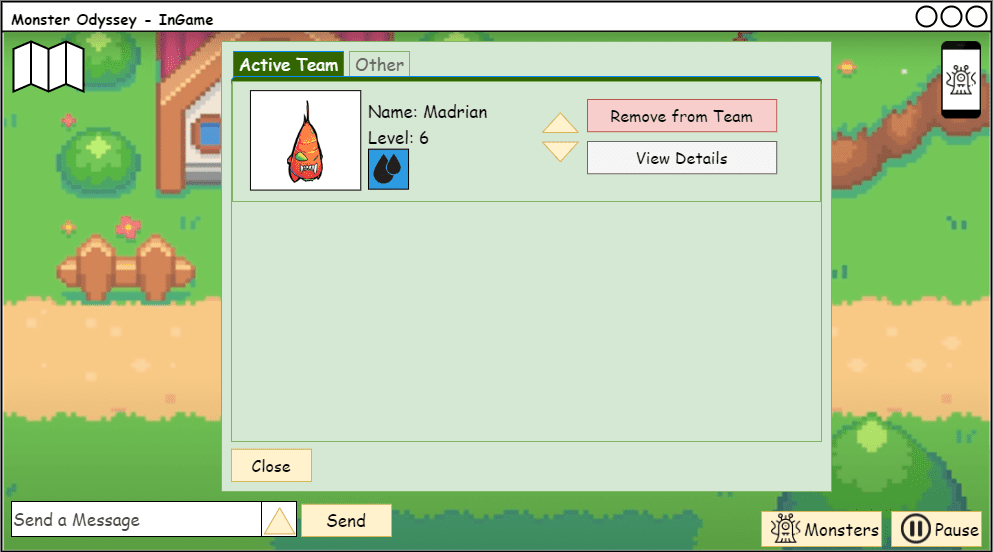
\includegraphics[width=\textwidth]{images/mockups/Monster/IngameMonsterMonsterActiveWithoutFlamurtle.png}
        \caption{Mockup: Aktives Monsterteam \phantom{aaa}}
        \label{fig: Mockup: Aktives Monsterteam}
    \end{subfigure}
    \hfill
    \begin{subfigure}[b]{0.4\textwidth}
        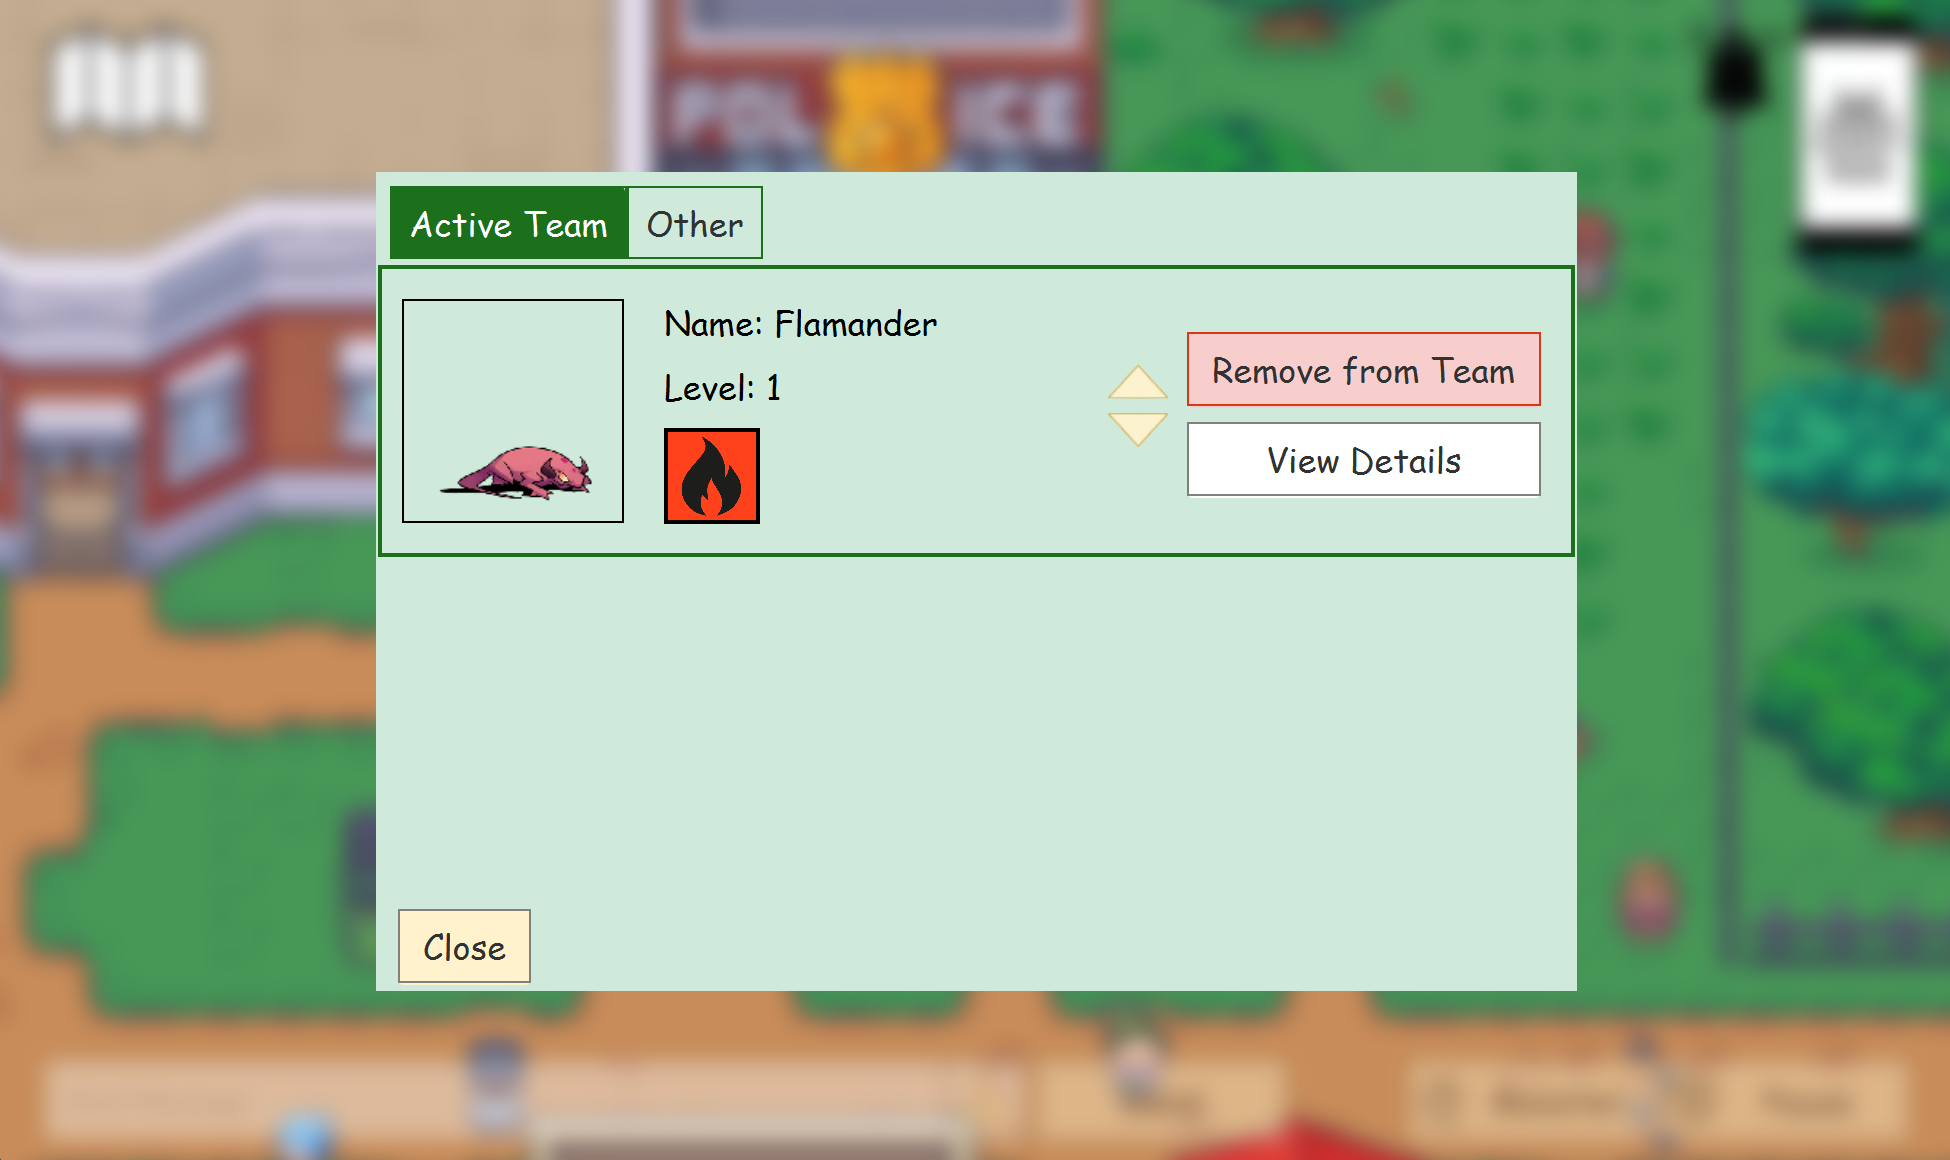
\includegraphics[width=\textwidth]{images/implementation/Monster/Monsterteam Active.png}
        \caption{Implementierung: Aktives Monsterteam}
        \label{fig: Implementierung: Aktives Monsterteam}
    \end{subfigure}
    \caption{Vergleich: Monsterliste}
    \label{fig: Vergleich: Monsterliste}
\end{figure}
Ferner sind in der Abbildung~\ref{fig: Vergleich: Monsterdetails} einige weitere Unterschiede anzumerken. Neu hinzugekommen in der Implementierung in der Abbildung~\ref{fig: Implementierung: Monsterdetails} ist der Monstername unter dem Monsterbild, der für die Monsterdetails wichtig ist. Außerdem sind Trennlinien zwischen den Balken und den links- und rechtsliegenden Elementen hinzugefügt worden, um die Struktur des Fensters klar darzustellen. Die Balken aus dem Mockup in der Abbildung~\ref{fig: Mockup: Monsterdetails} sind schmal und mit blauem Hintergrund ausgestattet, wobei die Balken in der Implementierung etwas größer und mit weißem Hintergrund gestaltet sind. Zu den jeweiligen Balken sind die Attribute in der Implementierung als Wort ausgeschrieben, um das jeweilige Attribut in die entsprechende Sprache übersetzen zu können, sodass die angebotenen Sprachen immer noch unterstützt werden.
Des Weiteren ist der Monstertyp oben rechts wie in der Abbildung~\ref{fig: Implementierung: Monsterdetails} festgelegt, da die Übersetzungen in den angebotenen Sprachen Platz in Anspruch nehmen.
Zuletzt sind die Fähigkeiten des Monsters noch weiter voneinander getrennt, was dennoch keine Funktionalitätsänderung mit sich führt.
\begin{figure}[H]
    \centering
    \begin{subfigure}[b]{0.4\textwidth}
        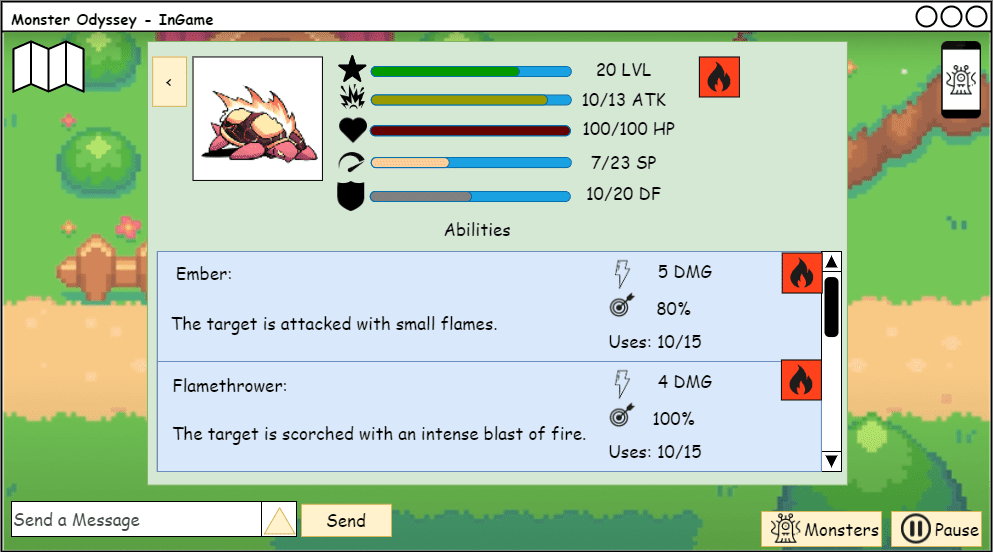
\includegraphics[width=\textwidth]{images/mockups/Monster/IngameMonsterDetails.png}
        \caption{Mockup: \phantom{aaamonsterr} Monsterdetails}
        \label{fig: Mockup: Monsterdetails}
    \end{subfigure}
    \hfill
    \begin{subfigure}[b]{0.4\textwidth}
        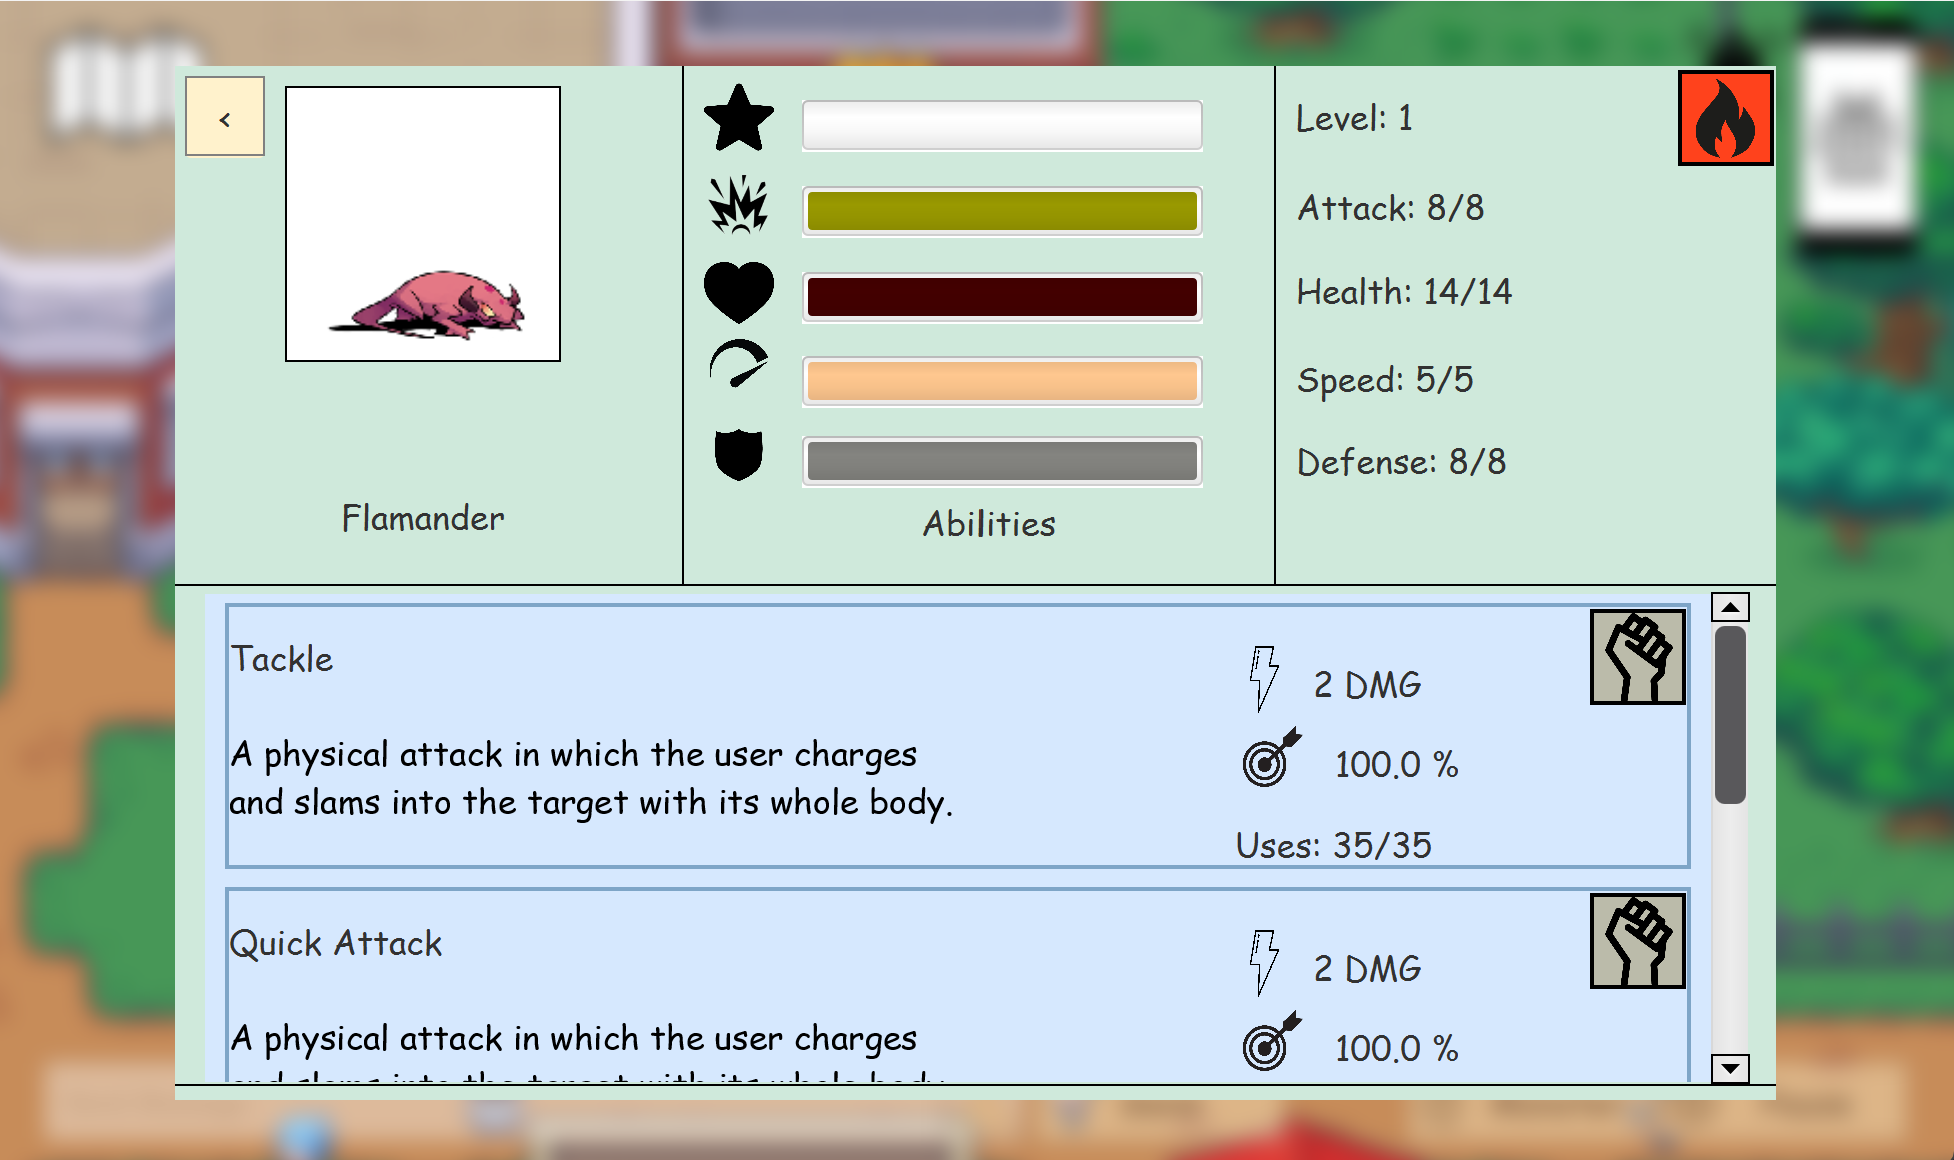
\includegraphics[width=\textwidth]{images/implementation/Monster/Monsterdetails .png}
        \caption{Implementierung: Monsterdetails}
        \label{fig: Implementierung: Monsterdetails}
    \end{subfigure}
    \caption{Vergleich: Monsterdetails}
    \label{fig: Vergleich: Monsterdetails}
\end{figure}